%************************************************
\chapter{Contexto y Estado del Arte}\label{ch:estadodelarte}

\section{Introducción}\label{sec:intro_estadodelarte}
\lipsum[1]

\section{Sección}\label{sec:produccion_estadodelarte}
\lipsum[1]~\cite{Becerra15,Castellanos14}.

\begin{figure}[h]
    \centering
    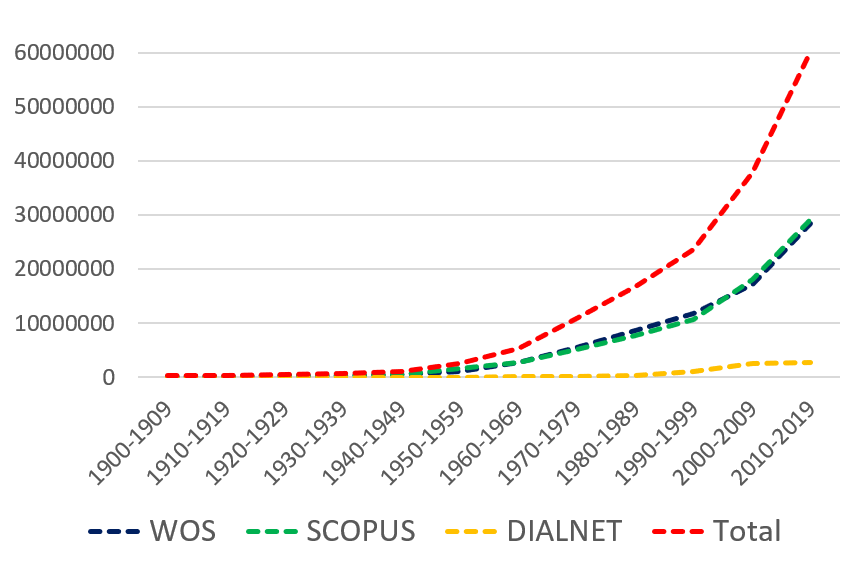
\includegraphics[width=\textwidth]{Figure/Imagen1}
    \caption{Volumen de producción científica en \ac{BDB}s}
    \label{fig:Imagen1}
\end{figure}

\lipsum[1]\ac{BDB}.

\section{Otra sección}\label{sec:bases_estadodelarte}
\lipsum[1-4]

\section{Contexto}\label{sec:contexto_estadodelarte}
\lipsum[2-3]

El \ac{MES} ha sido sistemático en la evaluación de indicadores relacionados con la producción científica en las universidades.
Las valoraciones son recogidas en un documento con carácter anual llamado: ``Informe de Balance de Ciencia e Innovación Tecnológica''. 
El mismo refleja, en el impacto científico tecnológico, el total de publicaciones por profesores y la cantidad que son publicadas en \ac{BDB} internacionales. 
Para hacer una diferencia en cuanto a la calidad de las publicaciones, se estableció una clasificación de publicaciones realizadas en revistas científicas según su origen de publicación:
\begin{itemize}
    \item \textbf{Grupo I:} Web of Science o SCOPUS
    \item \textbf{Grupo II:} bases de datos internacionales
    \item \textbf{Grupo III:} bases de datos iberoamericanas
    \item \textbf{Grupo IV:} revistas científicas acreditadas a nivel nacional
\end{itemize}

\subsection{Estudios Anteriores}\label{sec:estudios_estadodelarte}
\lipsum[1-2]